%! Author = welby
%! Date = 9/9/25

% Preamble
\documentclass[11pt]

% Packages
\usepackage{amsmath}
\usepackage{graphicx}

% Document
\begin{document}

    \begin{figure}[htbp]
        \centering

        % Row 1
        \begin{subfigure}{0.3\textwidth}
            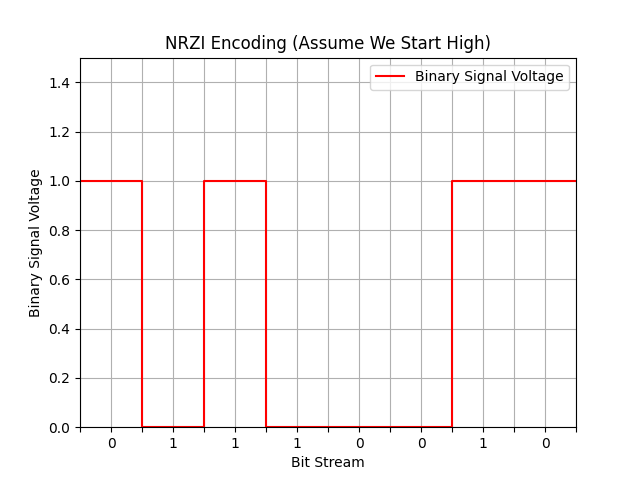
\includegraphics[width=\linewidth]{nrz}
            \caption{NRZ (Active Low)}
        \end{subfigure}
        \hfill
        \begin{subfigure}{0.3\textwidth}
            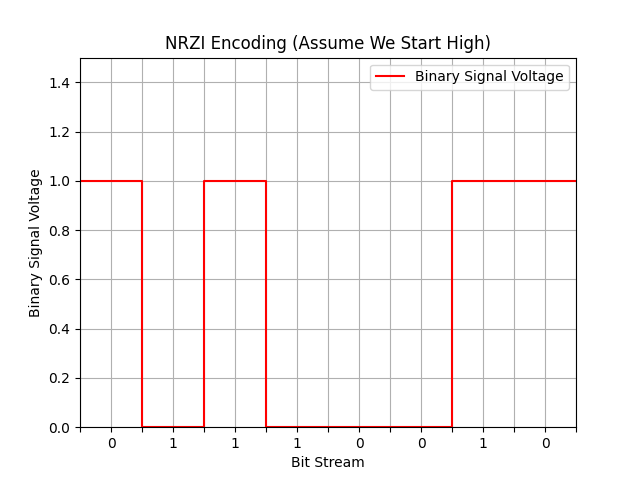
\includegraphics[width=\linewidth]{nrzi}
            \caption{NRZI}
        \end{subfigure}
        \hfill
        \begin{subfigure}{0.3\textwidth}
            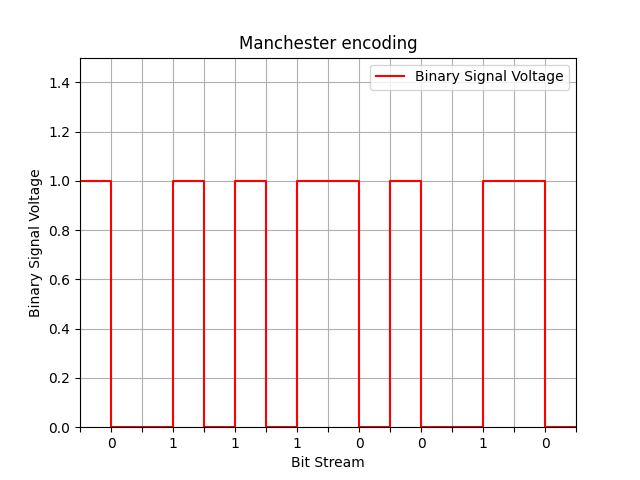
\includegraphics[width=\linewidth]{manchester}
            \caption{Manchester}
        \end{subfigure}

        \vspace{1em}

        % Row 2
        \begin{subfigure}{0.3\textwidth}
            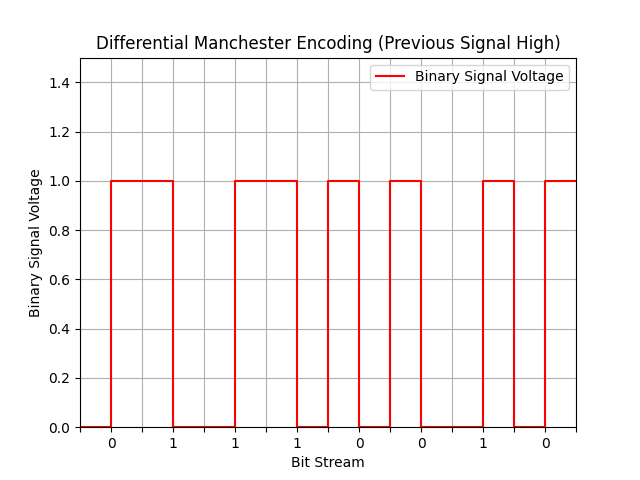
\includegraphics[width=\linewidth]{differential_manchester}
            \caption{Differential Manchester}
        \end{subfigure}
        \hfill
        \begin{subfigure}{0.3\textwidth}
            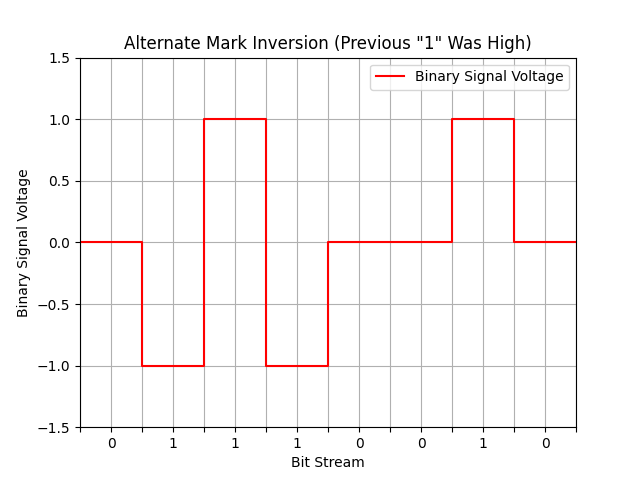
\includegraphics[width=\linewidth]{ami}
            \caption{AMI}
        \end{subfigure}
        \hfill
        \begin{subfigure}{0.3\textwidth}
            % empty slot, or you can drop this
        \end{subfigure}

        \caption{ NRZ, NRZI, Manchester, Differential Manchester, and AMI.}
    \end{figure}


\end{document}